% PRELIMINARY FINDINGS
\section{Early Findings} \label{skyfinds}

In this section, I present the results of my preliminary analysis. Before proceeding, we take a
moment to describe how closeness was obtained between \emph{labels}. This is most easily expressed
with the following illustrative example, where labels of interest are drawn from the
``country"-based labeling scheme (I trust that the reader can easily apply this method to AS
number, prefix, and /24): Consider two sets of clients from two countries, $P$ and $Q$. I perform
pairwise comparisons for all combinations containing exactly one client from each country.  From
this, I define the closeness of $P$ and $Q$ as the median of their set of client-pair closeness
scores. I use the median in an effort to avoid potentially noisy outlier behavior. Note, I allow
for $P$ and $Q$ to be the same label, as I am also interested in the closeness of clients in the
same group. All comparisons in this section use the described group aggregates for comparison. 

\begin{figure*}
    \center
            \begin{subfigure}[b]{.7\linewidth}
                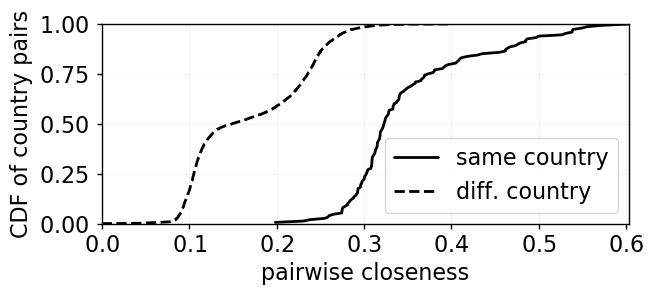
\epsfig{file=figs/country_cdf.png, width=1\linewidth}
                \caption{country}
            \end{subfigure}
            \begin{subfigure}[b]{.7\linewidth}
                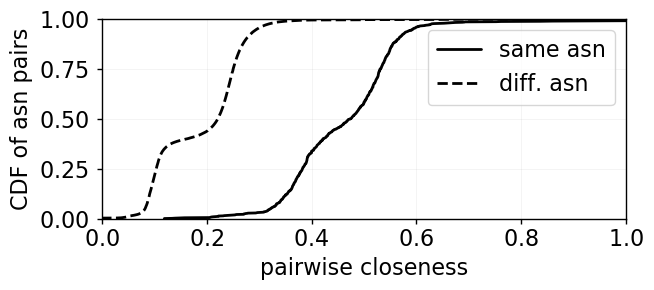
\epsfig{file=figs/asn_cdf.png, width=1\linewidth}
                \caption{asn}
            \end{subfigure}
            \begin{subfigure}[b]{.7\linewidth}
                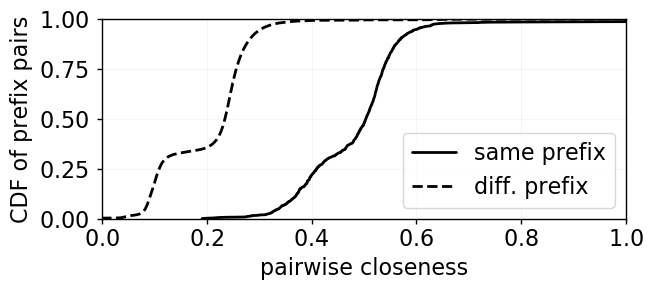
\epsfig{file=figs/prefix_cdf.png, width=1\linewidth}
                \caption{BGP prefix}
            \end{subfigure}
            \begin{subfigure}[b]{.7\linewidth}
                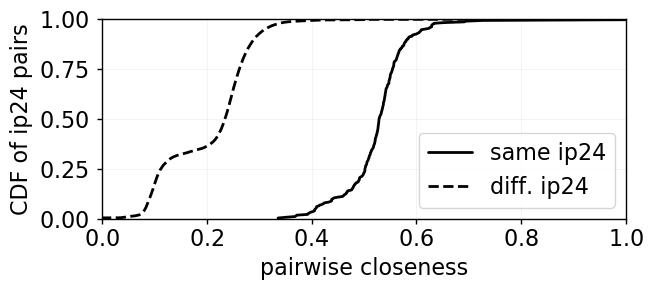
\epsfig{file=figs/ip24_cdf.png, width=1\linewidth}
                \caption{/24 subnet}
            \end{subfigure}
            \caption{CDFs of aggregate group closeness.}
            \label{closecdf}
\end{figure*}

Figure \ref{closecdf}, plots pairs of CDFs that contrast the closeness of clients in the same group with
that of different groups. Across all examined labeling schemes, clients in the same group tend to be
closer than those of different groups. However, the CDF pairs overlap to some extent, indicating
that there is generally no magic threshold at which we can assume clients to be in the same group.
More importantly, each curve spans over 30\% of possible closeness values, rendering it difficult
infer closeness based on matching or mismatching labels. It is possible that this is partially due
to the non-binary nature of the factors that determine closeness. Specifically, there likely a
gradient where closeness gradually increases or decreases as you move along some dimension in
client space. 

I draw attention to the fact that most of the observed closeness scores, even for clients in the
same /24, fell well below 1. This may partially stem from the fact that I define only DNS answers
with the \emph{same} /24 as a ``match" in closeness calculation. Such an approach makes each
comparison susceptible to the effects of load balancing and other dynamic labeling schemes. This
reflects the findings of previous work showing that even queries performed by the exact
same client may span a large range of possible answers, particularly for popular domains, CITE. 
\begin{figure*}
    \center
        \mbox{
            \begin{subfigure}[b]{.5\linewidth}
                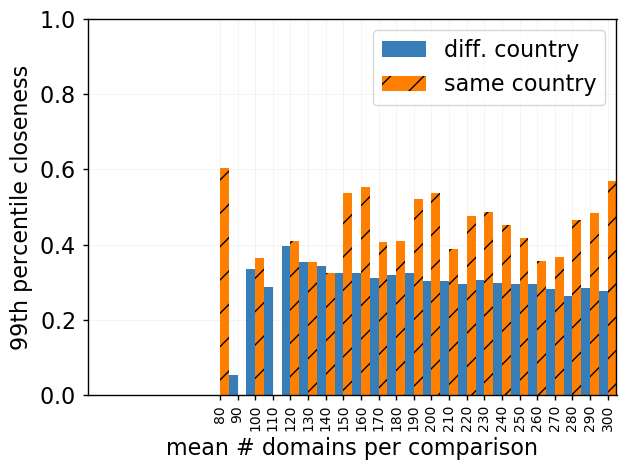
\epsfig{file=figs/country_percentile_vs_counts.png, width=1\linewidth}
                \caption{country}
            \end{subfigure}
            \begin{subfigure}[b]{.5\linewidth}
                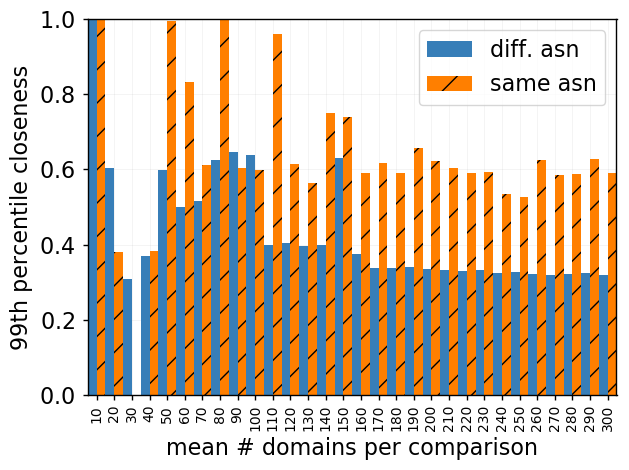
\epsfig{file=figs/asn_percentile_vs_counts.png, width=1\linewidth}
                \caption{asn}
            \end{subfigure}
        }
        \mbox{
            \begin{subfigure}[b]{.5\linewidth}
                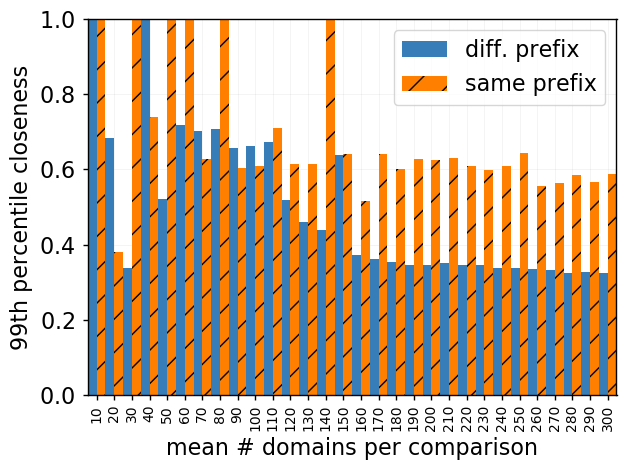
\epsfig{file=figs/prefix_percentile_vs_counts.png, width=1\linewidth}
                \caption{BGP prefix}
            \end{subfigure}
            \begin{subfigure}[b]{.5\linewidth}
                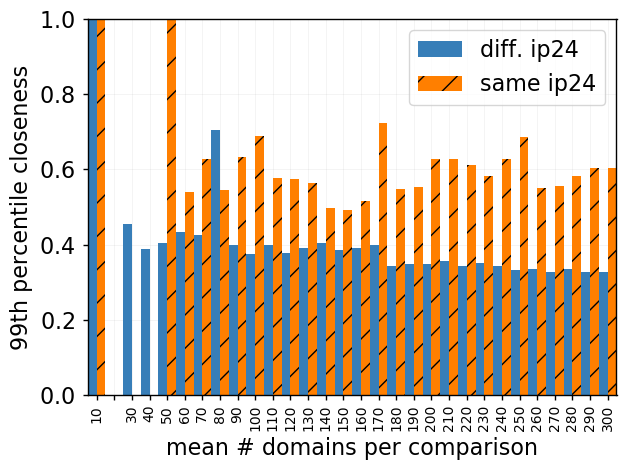
\epsfig{file=figs/ip24_percentile_vs_counts.png, width=1\linewidth}
                \caption{/24 subnet}
            \end{subfigure}
        }
            \caption{Bar plots of aggregate group closeness vs number of average number of domains
            used in closeness calculation for group pair.}
            \label{closecount}
\end{figure*}

As explained in Section \ref{closeness}, the size of $d$, the set of domains compared, varies across client
pairs. Figure \ref{closecount} shows how closeness scores for label pairs change with respect to the
average $d$ of their respective client pairs. Each bar correspends to a bin where $d$ ranges from
$x-10$ to $x$, and the height of the bar is the 99th percentile of all group aggregate pair scores
in that bin. Unlabeled tickmarks and bars with height 0 indicate empty bins (not zero values). I make the following
two observations. First, I see that as the number of domains compared increases, the closeness of
distinct labels \emph{decreases}; in other words, it becomes more apparent that clients are in
different groups as more domains are introduced to the closeness calculation. It is worth noting
however, that there seems to be a decrease in the marginal effect of each additional domain. Second,
I observe that closeness of clients with the same label \emph{stabilizes} after some number of
domains have been compared; it ceases to follow any general upward or downward trend.

Interestingly, in Figure \ref{closecount} it becomes acutely apparent that closeness does not
tend to increase with finer group granularity when using conventional groups. Although the closeness
of clients in the same country does exhibit slightly lower closeness scores, clients that share AS
number are equally close to clients that share the same /24 prefix.


